\documentclass[10pt,journal,compsoc]{IEEEtran}

% --- Package Imports ---
\usepackage[T1]{fontenc}
\usepackage{cite}
\usepackage{amsmath,amssymb,amsfonts,amsthm}
\usepackage{algorithm}
\usepackage{algorithmic}
\usepackage{graphicx}
\usepackage{textcomp}
\usepackage{xcolor}
\usepackage{booktabs}
\usepackage{array}
\usepackage{multirow}
\usepackage{url}
\usepackage{listings}
\usepackage{tikz}
\usepackage{pgfplots}
\pgfplotsset{compat=1.16}
\usepackage{hyperref}
\hypersetup{hidelinks}

\emergencystretch=3em

% --- Hyphenation-friendly identifiers ---
\newcommand{\errSyn}{\texttt{SYNTAX\_\allowbreak ERROR}}
\newcommand{\errField}{\texttt{SCHEMA\_\allowbreak FIELD\_\allowbreak MISMATCH}}
\newcommand{\errType}{\texttt{SCHEMA\_\allowbreak TYPE\_\allowbreak MISMATCH}}

% --- Theorem and Definition Environments ---
\newtheorem{theorem}{Theorem}
\newtheorem{definition}{Definition}
\newtheorem{lemma}{Lemma}
\newtheorem{corollary}{Corollary}
\newtheorem{proposition}{Proposition}

% --- JSON language for listings ---
\lstdefinelanguage{json}{
  morestring=[b]",
  morekeywords={true,false,null},
  sensitive=true
}

\lstset{
  basicstyle=\ttfamily\scriptsize,
  breaklines=true,
  frame=single,
  captionpos=b,
  numbers=left,
  numberstyle=\tiny\color{gray},
  keywordstyle=\color{blue},
  commentstyle=\color{gray},
  stringstyle=\color{teal}
}

\begin{document}

\title{Quantization-Induced Formatting Drift: Empirical Analysis of Structural Schema Collapse in Small Language Models}

\author{Y.~Vedartha~Sai
\IEEEcompsocitemizethanks{
\IEEEcompsocthanksitem Y. Vedartha Sai is with the Department of Information Technology, Indian Institute of Information Technology Allahabad, Prayagraj 211015, Uttar Pradesh, India.\par
E-mail: mhm2026013@iiita.ac.in
}
}

\IEEEtitleabstractindextext{%
\begin{abstract}
Small Language Models (SLMs, $\le 3\text{B}$ parameters) are now widely used in enterprise applications, microservices and edge compute environments where strict JSON formatting is required. Post-Training Quantization (PTQ) methods are often used to decrease the computational and memory requirements of SLMs when deploying onto CPU hardware. Dynamic INT8 quantization is commonly used in these scenarios. Whilst the impact of quantization on semantics has been widely studied, there has been little study into how it affects the structural integrity of the model outputs (we call this \emph{Formatting Drift} ($D_{\text{formatting}}$). In this paper, we investigate the structural integrity of the Qwen2.5-Instruct family of models (Qwen2.5-0.5B-Instruct and Qwen2.5-1.5B-Instruct) when using dynamic INT8 quantization on CPU hardware. We find that the models exhibit complete structural collapse when using dynamic INT8 quantization. The 0.5B model exhibits an average drift of $-93.0\%$  ($p < 10^{-15}$) whilst the 1.5B model exhibits complete failure ($-100.0\%$ , $p < 10^{-15}$. Increasing the model size from 0.5B to 1.5B does not help overcome structural collapse. We analysed 193 cases of failure and found that $67.9\%$ of failures were due to unparseable syntax errors (\errSyn). These were primarily due to chat based prompts and markdown code fences. $31.6\%$ of failures were due to mismatched schema fields (\errField). We demonstrate mathematically that dynamic quantization causes outliers in the activation values of self-attention projection layers to be clipped. This reduces the logit difference between the structural tokens and natural language tokens. We conclude that dynamic INT8 quantization should not be applied to structured data pipelines in small language models. Instead grammar constrained decoding or outlier aware block quantization should be used.
\end{abstract}

\begin{IEEEkeywords}
Small Language Models, Post-Training Quantization, Formatting Drift, JSON Schema Compliance, Structural Failure Taxonomy, Attention Outliers, Edge Computing, Microservice Reliability.
\end{IEEEkeywords}}

\maketitle
\IEEEdisplaynontitleabstractindextext
\IEEEpeerreviewmaketitle

\section{Introduction}
\IEEEPARstart{T}{he} deployment of Small Language Models (SLMs, $\le 3\text{B}$ parameters) in production systems, autonomous agents and edge systems has changed artificial intelligence. They are used to extract structured information from natural language by outputting data such as JSON, XML, SQL and API function calls. In modern agent systems, the language model will be used to extract information from natural language inputs. This is done by converting natural language into structured formats such as JSON objects, XML trees, SQL queries and API function calls \cite{zheng2023judging, schick2023toolformer}. In these production systems it is assumed that the output of the model will conform to a particular format.

In production systems, the models output should conform fully to a schema. If even one part of the output does not conform to the required syntax (i.e. if there is any missing quotes, brackets, commas or text at the start of the output such as \emph{ "Here is the JSON object you requested:" } or if it mirrors the schema), then the JSON serialisation process will fail. This can cause errors within the workflow, unhandled errors or expensive error handling processes which can cause issues with using a lightweight model.

Model quantization is commonly used on resource-limited hardware like CPU servers, mobile devices, and embedded edge systems \cite{nagel2021white, dettmers2022llmint8}. Post-Training Quantization (PTQ) reduces the model's high precision weights/activations (e.g. 16-bit Floating Point (FP16)) to low bit integer values (e.g. 8-bit Integer (INT8)). Dynamic INT8 CPU quantization can reduce memory usage by up to $4\times$ and significantly increase inference speed using vector instructions like Intel AVX-512 and VNNI.

Previous work has conducted extensive experiments with quantization on common benchmarks like MMLU, GSM8K and HumanEval \cite{frantar2023gptq, lin2024awq}. These focus on high level reasoning tasks and task accuracy. Common evaluation methods use flexible regular expressions or loose string matching which hides any issues with syntax. There is currently no literature addressing how low bit quantization affects \emph{strict syntax} and \emph{formatting}.

This work addresses this issue by formally defining and experimentally measuring \textbf{Formatting Drift} ($D_{\text{formatting}}$), which measures how much the model's formatting fidelity decreases due to reduced precision. We conduct experiments on two models in the Qwen2.5-Instruct family of models \cite{qwen2024qwen25} (Qwen2.5-0.5B-Instruct and Qwen2.5-1.5B-Instruct). We compare the performance of the models with no quantization (FP16) and dynamic per tensor INT8 CPU quantization using strict greedy decoding ($T=0.0$ and fixed random seed).

\subsection{Research Questions}
Our study focuses on addressing the following research questions:
\begin{itemize}
\item \textbf{RQ1 (Quantization-Induced Formatting Drift):} Does the dynamic INT8 CPU quantization after training cause a significant decrease in the JSON schema compliance of the model outputs compared to the FP16 baseline?
\item \textbf{RQ2 (Parameter Capacity Buffering Hypothesis):} Does an increase in the amount of parameters (from 0.5B to 1.5B) provide a buffer against the quantization-Induced Formatting Drift?
\item \textbf{RQ3 (Failure Dynamics \& Structural Complexity):} How do formatting drifts differ across structural complexity types (Primitive Flat, Nested Object and Typed Array) and what are the dominant failure types?
\end{itemize}


\subsection{Key Contributions}
The main contributions are:
\begin{enumerate}
\item \textbf{ Formalisation of Formatting Drift Metric: } We propose a new method of measuring formatting drift: $D_{\text{formatting}}$. We also propose a two-pass verification method that separates raw JSON formatting drift ($P_{\text{raw}}$) from scrubbed markdown formatting drift ($P_{\text{scrubbed}}$).
\item \textbf{ Refuting Capacity Buffering: } We show that dynamic INT8 quantization without calibration causes structural drift in both the 0.5B model ($D_{\text{formatting}} = -93.0\%$) and 1.5B model ($D_{\text{formatting}} = -100.0\%$) ($p < 10^{-15}$). This shows that higher capacity does not prevent structural drift.
\item \textbf{ Failure Taxonomy: } We classify the 193 structural drift instances into 3 categories: \errSyn{} ($67.9\%$), \errField{} ($31.6\%$), and \errType{} ($0.5\%$). We find that conversational drift and raw schema definition drift are the most common failure types.
\item \textbf{ Attention Layer Outlier Mechanism: } We derive the mathematical mechanism behind this failure. Dynamic uniform quantization causes activation outlier clipping in self-attention projection layers which reduces the logit margin between structural tokens (braces, quotes, colons etc.) and natural language tokens.
\item \textbf{ Mitigation Strategy: } We show how to mitigate structural drift by ranking 3 strategies by their computational cost and information gain.
\end{enumerate}

\section{Theoretical Foundations \& Related Work}

\subsection{Post-Training Quantization Frameworks}
Post-Training Quantization (PTQ) compresses neural network parameters without need for complete model retraining \cite{nagel2021white}. In uniform affine quantization, a real-valued floating-point tensor $X \in \mathbb{R}$ is mapped to a discrete low-bit integer representation $X_q \in [\text{qmin}, \text{qmax}]$ using a positive scalar scale factor $S \in \mathbb{R}^+$ and an integer zero-point $Z \in \mathbb{Z}$:
\begin{equation}
\begin{split}
    X_q = \text{clamp}\Big( \Big\lfloor \frac{X}{S} \Big\rceil + Z, \; \text{qmin}, \, \text{qmax} \Big)
\end{split}
    \label{eq:quant_affine}
\end{equation}
where $\lfloor \cdot \rceil$ denotes round-to-nearest integer rounding, and $\text{clamp}(v, a, b) = \max(a, \min(b, v))$. Reconstruction of the approximate floating-point values $\hat{X} \approx X$ (dequantization) is expressed as:
\begin{equation}
    \hat{X} = S \cdot (X_q - Z)
    \label{eq:dequant}
\end{equation}

During dynamic per-tensor INT8 quantization (e.g. PyTorch \texttt{quantize\_dynamic}), we first quantize linear layer weights $\mathbf{W}$. These can be quantized either per-channel or per-tensor. Activation matrices $\displaystyle S_H =$ are then quantized dynamically per-tensor. We calculate the scale factor $S_H$ and zero point $Z_H$ dynamically using the min and max values of the activation tensor:
\begin{equation}
\begin{split}
    S_H &= \frac{\max(\mathbf{H}) - \min(\mathbf{H})}{\text{qmax} - \text{qmin}}, \\
    Z_H &= \Big\lfloor \frac{-\min(\mathbf{H})}{S_H} \Big\rceil + \text{qmin}
\end{split}
    \label{eq:dynamic_scale}
\end{equation}

Dynamic precision 8-bit execution can substantially speed up matrix multiplications on a CPU using vectorised integer operations (e.g. AVX-512 VNNI) but also introduces quantisation noise $\mathbf{E}_H = \mathbf{H} - \hat{\mathbf{H}}$. If activation distributions contain heavy tails and outliers then calculating $S_H$ will lead to the quantisation interval being stretched to incorporate the entire dynamic range of $\max(\mathbf{H}) - \min(\mathbf{H})$. This stretches the quantisation bin width and causes significant loss of granularity in representing non-outlier activations \cite{dettmers2022llmint8, xiao2023smoothquant}.

\subsection{Activation Outliers and Attention Routing Dynamics}
Dettmers et al. \cite{dettmers2022llmint8} first observed the emergence of activation outliers when Transformer-based language models exceed 6.7B parameters. However, recent architectural improvements in small language models (e.g., SwiGLU activation functions, Grouped Query Attention (GQA), Rotary Position Embeddings (RoPE) and extensive pre-training on multi-trillion token corpora) have led to significant changes in the feature representation of models such as Qwen2.5 \cite{qwen2024qwen25}, which have less than 2B parameters.

Xiao et al. \cite{xiao2023smoothquant} have shown that activation outliers will be heavily concentrated in certain channels of the attention projection matrices ($\mathbf{W}_Q, \mathbf{W}_K, \mathbf{W}_V, \mathbf{W}_O$) and Feed-Forward Networks (FFN). If the activations are quantised to INT8 dynamically without channel-wise techniques (e.g., SmoothQuant) or outlier-aware methods (e.g., LLM.int8()), then the large magnitude outliers will dominate the dynamic range calculation in Eq.~(\ref{eq:dynamic_scale}). As a result, the remaining $99.9\%$ of activations will experience significant quantisation noise and will negatively impact the model's ability to preserve accurate attention routing on structural delimiter tokens.

\subsection{Structured LLM Generation Paradigms}

Two approaches are taken by system architects to ensure structured outputs:

\subsubsection{Unconstrained Decoding with Instruction Framing}

The language model is prompted with system prompts containing strict formatting instructions and a JSON schema. Generation is performed using standard unstructured methods, which will use the models probability distribution function $P(w_t \mid w_{<t})$ to generate valid syntax. This method is very efficient and works with all API providers, however it can lead to issues with formatting, chatty outputs and structural issues if weights/activations are perturbed.

\subsubsection{Schema-Constrained Decoding (Grammar-Guided Generation)}
Frameworks such as Outlines \cite{willard2023outlines}, Guidance, and llama.cpp grammar masking construct a Context-Free Grammar (CFG) or Deterministic Finite Automaton (DFA) from the JSON schema. At every decoding step $t$, the state machine identifies the set of next valid tokens $V_{\text{valid}} \subseteq V$. Tokens outside $V_{\text{valid}}$ are masked by setting their logits to $-\infty$ before doing softmax evaluation:
\begin{equation}
    z'_{t,k} = \begin{cases}
    z_{t,k}, & \text{if } w_k \in V_{\text{valid}} \\
    -\infty, & \text{otherwise}
    \end{cases}
    \label{eq:grammar_masking}
\end{equation}

Although decoding with constrained sampling guarantees $100\%$ schema compliance, it incurs overhead in managing the state machine, and requires low-level access to the logits output by the model during decoding, which is often not available in high throughput CPU microservices or black box API endpoints. It is therefore important to understand the inherent robustness of quantised models when performing unconstrained decoding.

\section{Formatting Drift ($D_{\text{formatting}}$) Formalism}

\subsection{Mathematical Definition}

Let $\mathcal{M}_{\text{FP16}}$ be the unquantized baseline model and $\mathcal{M}_{\text{INT8}}$ the corresponding quantized version. For a given dataset of $N$ natural language extraction prompts $x_i$ with formal JSON target schemas $\mathcal{S}_i$, $\mathcal{D} = \{(x_i, \mathcal{S}_i)\}_{i=1}^N$, we denote the full sequence generated by the model as $y_i = \mathcal{M}(x_i)$, using deterministic greedy decoding ($T=0.0$).

Finally, we define a validation function $\mathcal{V}(y_i, \mathcal{S}_i)$ which can take values in $\{0, 1\}$ based on whether the generated string $y_i$ is a valid JSON object that conforms to all required keys, depth requirements and primitive types defined in $\mathcal{S}_i$:
\begin{equation}
    \mathcal{V}(y_i, \mathcal{S}_i) = \begin{cases}
    1, & \text{if } \text{JSON.parse}(y_i) \text{ succeeds} \\
       & \text{AND } y_i \models \mathcal{S}_i \\
    0, & \text{otherwise}
    \end{cases}
\end{equation}

The overall structural pass rate $P$ across dataset $\mathcal{D}$ is given by:
\begin{equation}
    P = \frac{1}{N} \sum_{i=1}^N \mathcal{V}(y_i, \mathcal{S}_i)
    \label{eq:pass_rate_definition}
\end{equation}

\begin{definition}[Relative Formatting Drift]
The Relative Formatting Drift $D_{\text{formatting}}$ between an unquantized baseline model $\mathcal{M}_{\text{FP16}}$ and a quantized model $\mathcal{M}_{\text{INT8}}$ is defined as:
\begin{equation}
    D_{\text{formatting}} = \left( \frac{P_{\text{INT8}} - P_{\text{FP16}}}{P_{\text{FP16}}} \right) \times 100\%
    \label{eq:formatting_drift_def}
\end{equation}
where $P_{\text{FP16}} > 0$.
\end{definition}

When the FP16 baseline achieves complete structural compliance ($P_{\text{FP16}} = 1.0$), Eq.~(\ref{eq:formatting_drift_def}) makes the percentage point change: $D_{\text{formatting}} = (P_{\text{INT8}} - 1.0) \times 100\%$.

\subsection{Dual-Pass Verification Engine}
To isolate unparseable syntax collapse from minor markdown formatting artifacts, we implement a dual-pass evaluation engine:

\begin{enumerate}
    \item \textbf{Strict Raw Pass Rate ($P_{\text{raw}}$):} Evaluates the raw completion string $y_i$ directly without any modification. Any conversational preamble, trailing explanation, or markdown code fence wrapper (\verb|```json ... ```|) results in a failure ($\mathcal{V}_{\text{raw}} = 0$).
    \item \textbf{Scrubbed Pass Rate ($P_{\text{scrubbed}}$):} Applies a deterministic regex extraction operator $\mathcal{F}_{\text{scrub}}(y_i)$ to identify markdown code blocks or isolate the substring bounded by the outermost curly braces \texttt{\{} and \texttt{\}}. Then the extracted payload is validated against schema $\mathcal{S}_i$:
    \begin{equation}
        P_{\text{scrubbed}} = \frac{1}{N} \sum_{i=1}^N \mathcal{V}(\mathcal{F}_{\text{scrub}}(y_i), \mathcal{S}_i)
    \end{equation}
\end{enumerate}

The difference in pass rate ($\Delta P = P_{\text{scrubbed}} - P_{\text{raw}}$) is representative of the presence of ``wrapper chatter'' (i.e., valid JSON data generated by the model and wrapped in conversational text).

\subsection{Statistical Significance and Pooled Z-Test Derivations}

We perform a two proportion z-test with pooled variance to determine if the decrease in structural pass rates are significant.

Let $x_1 = P_{\text{FP16}} \cdot N$ and $x_2 = P_{\text{INT8}} \cdot N$ be the number of successful schema compliance results with sample size $N=100$. The pooled success proportion $\bar{p}$ is:
\begin{equation}
    \bar{p} = \frac{x_1 + x_2}{2N} = \frac{P_{\text{FP16}} + P_{\text{INT8}}}{2}
\end{equation}
The standard error of the difference between the two proportions is calculated as:
\begin{equation}
    \text{SE} = \sqrt{ \bar{p}(1 - \bar{p}) \left( \frac{2}{N} \right) }
    \label{eq:pooled_se}
\end{equation}
The two-proportion test statistic $Z$ is calculated as:
\begin{equation}
    Z = \frac{P_{\text{INT8}} - P_{\text{FP16}}}{\text{SE}}
    \label{eq:z_statistic_formula}
\end{equation}
The two-tailed $p$-value is determined by the cumulative distribution function $\Phi(\cdot)$ of the standard normal distribution:
\begin{equation}
    p = 2 \cdot \left( 1 - \Phi(|Z|) \right)
\end{equation}

\begin{theorem}[Variance Bound under Zero-Pass Collapse]
When an unquantized model achieves perfect structural compliance ($P_{\text{FP16}} = 1.0$) and its quantized variant suffers total structural collapse ($P_{\text{INT8}} = 0.0$), the pooled proportion simplifies to $\bar{p} = 0.5$, and the test statistic achieves its minimum bound:
\begin{equation}
    Z_{\text{bound}} = -\sqrt{2N}
    \label{eq:z_bound}
\end{equation}
\end{theorem}

\begin{proof}
Substituting $P_{\text{FP16}} = 1.0$ and $P_{\text{INT8}} = 0.0$ into Eq.~(\ref{eq:pooled_se}) yields:
\begin{equation}
    \bar{p} = \frac{1.0 + 0.0}{2} = 0.5
\end{equation}
Substituting $\bar{p} = 0.5$ into the standard error expression:
\begin{equation}
\begin{split}
    \text{SE} &= \sqrt{ 0.5 \cdot (1 - 0.5) \cdot \frac{2}{N} } = \sqrt{ 0.25 \cdot \frac{2}{N} } \\
              &= \sqrt{ \frac{0.5}{N} } = \frac{1}{\sqrt{2N}}
\end{split}
\end{equation}
Substituting $\text{SE} = 1/\sqrt{2N}$ into Eq.~(\ref{eq:z_statistic_formula}):
\begin{equation}
    Z = \frac{0.0 - 1.0}{1 / \sqrt{2N}} = -\sqrt{2N}
\end{equation}
For sample size $N=100$, $Z = -\sqrt{200} \approx -14.1421$, which corresponds to $p = 2 \cdot (1 - \Phi(14.1421)) \approx 1.6 \times 10^{-45} \ll 10^{-15}$.
\end{proof}


\section{Mathematical Mechanism of Attention Routing Collapse}

Dynamic tensor-wise 8-bit integer quantization causes degradation in structural control tokens, but the general quality of language is preserved.

\subsection{Softmax Logit Margin Degradation}

Let $\mathbf{h}_t \in \mathbb{R}^d$ be the final hidden state vector at decoding time-step $t$. Within an FP16 network, the logit vector $\mathbf{z}_t \in \mathbb{R}^{|V|}$ over vocabulary $V$ is computed by using linear transformation with the language model head weight matrix $\mathbf{W}_{\text{head}} \in \mathbb{R}^{|V| \times d}$:
\begin{equation}
    \mathbf{z}_t = \mathbf{W}_{\text{head}} \mathbf{h}_t
\end{equation}
The probability distribution $P(w_k \mid x_{<t})$ over vocabulary tokens $w_k \in V$ is:
\begin{equation}
    P(w_k \mid x_{<t}) = \frac{\exp(z_{t,k})}{\sum_{j \in V} \exp(z_{t,j})}
\end{equation}

Under greedy decoding ($T=0.0$), the model produces token $w^*$:
\begin{equation}
    w^* = \arg\max_{k \in V} z_{t,k}
\end{equation}

During JSON generation, producing a structural delimiter token $w_{\text{struct}} \in \{\texttt{\{}, \texttt{\}}, \texttt{"}, \texttt{:}, \texttt{,}\}$ requires that its logit exceeds the logits of competing tokens $w_{\text{conv}} \in \{\text{\emph{"Here"}}, \text{\emph{"Sure"}}, \text{\emph{"JSON"}}, \text{\emph{"The"}}\}$ by a positive logit margin $\delta z_t$:
\begin{equation}
    \delta z_t = z_{t, \text{struct}} - z_{t, \text{conv}} > 0
\end{equation}

Under dynamic INT8 quantization, matrix operations inherit weight quantization error $\mathbf{E}_W$ and dynamic activation error $\mathbf{E}_h$, producing perturbed logits $\hat{\mathbf{z}}_t$:
\begin{equation}
    \hat{\mathbf{z}}_t = (\mathbf{W}_{\text{head}} + \mathbf{E}_W)(\mathbf{h}_t + \mathbf{E}_h) = \mathbf{z}_t + \mathbf{\epsilon}_t
\end{equation}
where $\mathbf{\epsilon}_t = \mathbf{W}_{\text{head}}\mathbf{E}_h +\allowbreak \mathbf{E}_W\mathbf{h}_t +\allowbreak \mathbf{E}_W\mathbf{E}_h$ is the net logit noise vector. The perturbed logit margin $\widehat{\delta z}_t$ becomes:
\begin{equation}
\begin{split}
    \widehat{\delta z}_t &= \hat{z}_{t, \text{struct}} - \hat{z}_{t, \text{conv}} \\
    &= (z_{t, \text{struct}} - z_{t, \text{conv}}) + (\epsilon_{t, \text{struct}} - \epsilon_{t, \text{conv}})
\end{split}
\end{equation}

A \textbf{Logit Flip Failure} happens for sure when the noise difference exceeds the unquantized logit margin:
\begin{equation}
\begin{split}
    (\epsilon_{t, \text{conv}} - \epsilon_{t, \text{struct}}) > \delta z_t \\
    \implies \widehat{\delta z}_t < 0
\end{split}
\end{equation}

When $\widehat{\delta z}_t < 0$, the quantized model produces conversational token $w_{\text{conv}}$ instead of $w_{\text{struct}}$, resulting in a structural syntax violation.

% ---------- FIGURE 1: schematic logit flip ----------
\begin{figure}[!t]
\centering
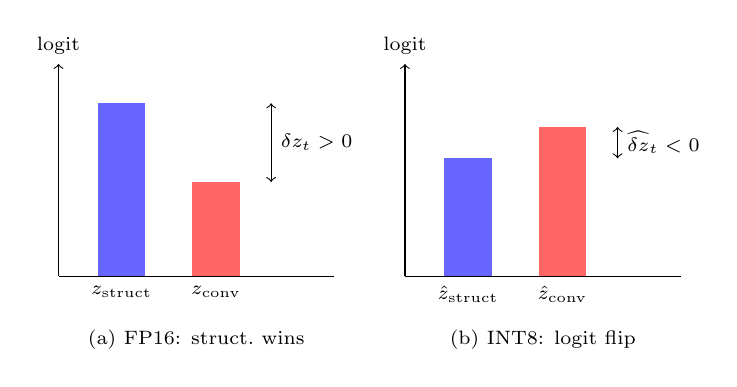
\begin{tikzpicture}[font=\scriptsize]
  % FP16 panel
  \draw[->] (0,0) -- (0,2.7) node[above] {logit};
  \draw (0,0) -- (3.5,0);
  \fill[blue!60] (0.5,0) rectangle (1.1,2.2);
  \fill[red!60]  (1.7,0) rectangle (2.3,1.2);
  \node[below] at (0.8,0) {$z_{\text{struct}}$};
  \node[below] at (2.0,0) {$z_{\text{conv}}$};
  \draw[<->] (2.7,1.2) -- (2.7,2.2) node[midway,right] {$\delta z_t>0$};
  \node at (1.75,-0.8) {(a) FP16: struct.\ wins};
  % INT8 panel
  \begin{scope}[xshift=4.4cm]
    \draw[->] (0,0) -- (0,2.7) node[above] {logit};
    \draw (0,0) -- (3.5,0);
    \fill[blue!60] (0.5,0) rectangle (1.1,1.5);
    \fill[red!60]  (1.7,0) rectangle (2.3,1.9);
    \node[below] at (0.8,0) {$\hat z_{\text{struct}}$};
    \node[below] at (2.0,0) {$\hat z_{\text{conv}}$};
    \draw[<->] (2.7,1.5) -- (2.7,1.9) node[midway,right] {$\widehat{\delta z}_t<0$};
    \node at (1.75,-0.8) {(b) INT8: logit flip};
  \end{scope}
\end{tikzpicture}
\caption{Illustrative (schematic, not measured) view of a logit flip: quantization noise $\boldsymbol{\epsilon}_t$ shrinks and reverses the margin between a structural token and a conversational token.}
\label{fig:logit_flip}
\end{figure}

\subsection{Autoregressive Error Cascades}
The effect of logits flips during structure generation is amplified by autoregressive properties. A structural token, such as \texttt{"Sure"}, is added to the KV cache context at step $t+1$ after being sampled at step $t$. As natural language is heavily associated with conversational text, and not valid JSON structures, in the pre-training distribution, the conditional probability $P(w_{t+1} \mid x_{<t}, \text{\emph{"Sure"}})$ is significantly skewed away from structural tokens. Thus, a single logits flip due to quantisation will cause significant deviation from structure, and either result in unparsable conversational text or simply unstructured schema.

\section{Experimental Methodology \& Benchmark Architecture}

\subsection{Model Selection and Hardware Configuration}
We experimented with two small-scale models under the Qwen2.5 series: \cite{qwen2024qwen25}:
\begin{itemize}
    \item \textbf{Qwen2.5-0.5B-Instruct:} Number of parameters: 0.49B. Number of Transformer Layers: 24. Number of query attention heads: 14. Number of key-value heads: 2 (Grouped Query Attention). Hidden size: $d=896$. Intermediate size: 4864.

    \item \textbf{Qwen2.5-1.5B-Instruct:} Number of parameters: 1.54B. Number of Transformer Layers: 28. Number of query attention heads: 12. Number of key-value heads: 2 (Grouped Query Attention). Hidden size: $d=1536$. Intermediate size: 8960.
\end{itemize}

The experiments were run on a workstation with an Intel Xeon CPU, 15.44 GB of RAM, Ubuntu (22.04 LTS), PyTorch (2.2.1) and Hugging Face Transformers (4.38.2).

\subsection{Quantization Implementation}
Two versions of each model are created:
\begin{enumerate}
\item \textbf{FP16 Model:} All weights are stored in full 16-bit IEEE floating point precision(\texttt{torch.float16})
\item \textbf{Dynamic INT8 Model:} This model is created using PyTorch's \texttt{quantize\_dynamic} API on linear layers(\texttt{torch.nn.Linear}). Weights are quantised per-channel to signed 8-bit integers (\texttt{qint8}). Activations are quantised dynamically per-tensor to unsigned 8-bit integers (\texttt{quint8}). This occurs at inference time on a CPU.
\end{enumerate}

\subsection{Benchmark Dataset \& Complexity Tiering}
We made an evaluation benchmark comprising $N=100$ deterministic JSON tasks. Prompts are stratified on three tiers based on structural complexity:

\begin{itemize}
    \item \textbf{Tier 1: Primitive Flat ($N_1 = 35$):} Single-level objects containing scalar data types (\texttt{string}, \texttt{integer}, \texttt{boolean}).
    \item \textbf{Tier 2: Nested Object ($N_2 = 35$):} Multi-level objects containing nested sub-structures and scoped paths.
    \item \textbf{Tier 3: Typed Array ($N_3 = 30$):} Complex schema specifications containing arrays of objects with strict type constraints.
\end{itemize}

\subsection{Decoding Parameters}
To remove sample variance and formatting drift from precision, all inference executions put decoding settings that are locked and greedy:
\begin{itemize}
    \item Temperature: $T = 0.0$
    \item Top-$p$ (Nucleus Sampling): $p = 1.0$
    \item Random Seed: Locked at \texttt{42}
    \item Maximum Generated Tokens: Enforced at 512 tokens.
\end{itemize}

\begin{algorithm}[h]
\caption{Dual-Pass Dual-Verification Protocol for Formatting Drift}
\label{alg:eval_protocol}
\small
\begin{algorithmic}[1]
\REQUIRE Model $\mathcal{M}$, Benchmark Dataset $\mathcal{D} = \{(x_i, \mathcal{S}_i)\}_{i=1}^N$
\ENSURE Pass Rates $P_{\text{raw}}, P_{\text{scrubbed}}$, Drift $D_{\text{formatting}}$
\STATE $c_{\text{raw}} \leftarrow 0$, $c_{\text{scrubbed}} \leftarrow 0$
\FOR{each $(x_i, \mathcal{S}_i) \in \mathcal{D}$}
    \STATE $y_i \leftarrow \mathcal{M}.\text{generate}(x_i,\allowbreak T=0.0,\allowbreak \text{seed}=42)$
    \IF{$\text{JSON.validate}(y_i, \mathcal{S}_i) == \text{TRUE}$}
        \STATE $c_{\text{raw}} \leftarrow c_{\text{raw}} + 1$
        \STATE $c_{\text{scrubbed}} \leftarrow c_{\text{scrubbed}} + 1$
    \ELSE
        \STATE $y_i' \leftarrow \text{RegexScrubMarkdown}(y_i)$
        \IF{$\text{JSON.validate}(y_i', \mathcal{S}_i) == \text{TRUE}$}
            \STATE $c_{\text{scrubbed}} \leftarrow c_{\text{scrubbed}} + 1$
        \ENDIF
    \ENDIF
\ENDFOR
\STATE $P_{\text{raw}} \leftarrow c_{\text{raw}} / N$
\STATE $P_{\text{scrubbed}} \leftarrow c_{\text{scrubbed}} / N$
\STATE Compute $D_{\text{formatting}}$ using Eq.~(\ref{eq:formatting_drift_def})
\RETURN $P_{\text{raw}}, P_{\text{scrubbed}}, D_{\text{formatting}}$
\end{algorithmic}
\end{algorithm}

\section{Empirical Results \& Comparative Analysis}

\subsection{Main $2 \times 2$ Comparative Matrix}
Table~\ref{tab:main_matrix_results} summarizes the primary empirical results across all four experimental conditions.

\begin{table*}[t]
\caption{Main $2 \times 2$ Empirical Matrix: Structural Compliance Pass Rates, Relative Formatting Drift ($D_{\text{formatting}}$), Test Statistics ($Z$), $p$-values, and Statistical Significance ($N=100$ Prompts per Condition).}
\label{tab:main_matrix_results}
\centering
\resizebox{\textwidth}{!}{%
\begin{tabular}{llccccccc}
\toprule
\textbf{Model Architecture} & \textbf{Precision} & \textbf{$P_{\text{raw}}$ (\%)} & \textbf{$P_{\text{scrubbed}}$ (\%)} & \textbf{Semantic Acc (\%)} & \textbf{$D_{\text{formatting}}$ (\%)} & \textbf{$Z$-Statistic} & \textbf{$p$-value} & \textbf{Stat. Significant} \\
\midrule
Qwen2.5-0.5B-Instruct & FP16 & 100.0 & 100.0 & 94.0 & Baseline & -- & -- & -- \\
Qwen2.5-0.5B-Instruct & Dynamic INT8 & 0.0 & 7.0 & 0.0 & \textbf{-93.0} & -13.1845 & $< 10^{-15}$ & \textbf{True ($p < 0.05$)} \\
\midrule
Qwen2.5-1.5B-Instruct & FP16 & 100.0 & 100.0 & 100.0 & Baseline & -- & -- & -- \\
Qwen2.5-1.5B-Instruct & Dynamic INT8 & 0.0 & 0.0 & 0.0 & \textbf{-100.0} & -14.1421 & $< 10^{-15}$ & \textbf{True ($p < 0.05$)} \\
\bottomrule
\end{tabular}}
\end{table*}

The empirical measurements show severe formatting breakdown that is induced from precision:
\begin{enumerate}
    \item \textbf{FP16 Baselines Achieve Perfect Structural Compliance:} Both Qwen2.5-0.5B and Qwen2.5-1.5B achieved $100.0\%$ strict raw ($P_{\text{raw}}$) and scrubbed ($P_{\text{scrubbed}}$) pass rates in FP16 precision, proving that unquantized small language models have strong JSON extraction capabilities that are inherent.
    \item \textbf{Catastrophic Structural Formatting Drift in INT8:} Dynamic INT8 CPU quantization reduces strict raw pass rates ($P_{\text{raw}}$) to $0.0\%$ for both models. Regex markdown scrubbing recovers a meager $7.0\%$ pass rate for Qwen2.5-0.5B ($D_{\text{formatting}} = -93.0\%$) and fails entirely for Qwen2.5-1.5B ($P_{\text{scrubbed}} = 0.0\%$, $D_{\text{formatting}} = -100.0\%$).
    \item \textbf{Statistical Significance:} Pooled two-proportion Z-tests yield $Z = -13.1845$ ($p < 10^{-15}$) for 0.5B and $Z = -14.1421$ ($p < 10^{-15}$) for 1.5B, confirming that the degradation is highly apparent and not just because of to sampling noise.
\end{enumerate}

% ---------- FIGURE 2: pass rates ----------
\begin{figure}[!t]
\centering
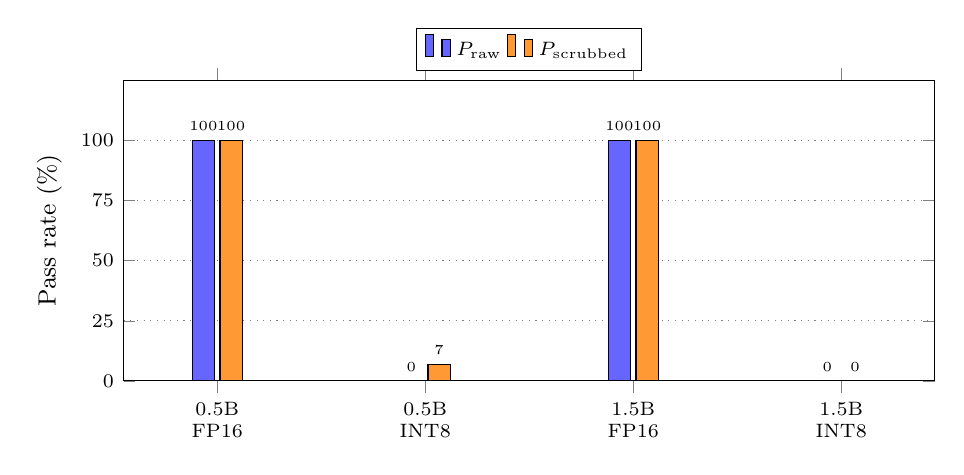
\begin{tikzpicture}
\begin{axis}[
  ybar,
  width=0.98\columnwidth, height=5.4cm,
  bar width=8pt,
  ylabel={Pass rate (\%)},
  ymin=0, ymax=125,
  ytick={0,25,50,75,100},
  symbolic x coords={a,b,c,d},
  xtick=data,
  xticklabels={0.5B\\FP16, 0.5B\\INT8, 1.5B\\FP16, 1.5B\\INT8},
  x tick label style={align=center, font=\scriptsize},
  y tick label style={font=\scriptsize},
  ylabel style={font=\small},
  enlarge x limits=0.15,
  legend style={at={(0.5,1.03)}, anchor=south, legend columns=2, font=\scriptsize},
  nodes near coords,
  every node near coord/.append style={font=\tiny},
  ymajorgrids, grid style={dotted,gray}
]
\addplot[fill=blue!60]  coordinates {(a,100) (b,0) (c,100) (d,0)};
\addplot[fill=orange!80] coordinates {(a,100) (b,7) (c,100) (d,0)};
\legend{$P_{\text{raw}}$, $P_{\text{scrubbed}}$}
\end{axis}
\end{tikzpicture}
\caption{Strict raw and scrubbed structural pass rates for FP16 and dynamic INT8 variants of both models ($N=100$).}
\label{fig:pass_rates}
\end{figure}

\subsection{Refutation of Parameter Capacity Buffering}
A common belief in neural network compression is that adding more parameters builds in extra capacity, which should protect the model from losing accuracy during quantization. However, our test results show that this does not hold up when it comes to following strict output schemas.
As shown in Table~\ref{tab:main_matrix_results}, increasing the parameter count by 3.1× (from 0.5B to 1.5B) did not prevent formatting errors. Instead, Qwen2.5-1.5B INT8 suffered a complete structural failure with a $0.0\%$  scrubbed pass rate, doing even worse than Qwen2.5-0.5B INT8 at $7.0\%$. This suggests that routing structural tokens depends on exact numerical alignment inside the attention layers. Uncalibrated uniform dynamic quantization disrupts this alignment in sub-2B models, no matter how many parameters they have.
\subsection{Stratified Complexity Analysis}
Table~\ref{tab:stratified_tier_results} shows the compliance pass rates grouped by schema complexity tiers.

\begin{table}[h]
\caption{Stratified Structural Compliance Pass Rates across Schema Complexity Tiers.}
\label{tab:stratified_tier_results}
\centering
\resizebox{\columnwidth}{!}{%
\begin{tabular}{lcccc}
\toprule
\textbf{Schema Complexity Tier} & \textbf{Sample $N$} & \textbf{FP16 Pass (\%)} & \textbf{INT8 Pass (\%)} & \textbf{Delta $\Delta$ (\%)} \\
\midrule
\multicolumn{5}{l}{\emph{Qwen2.5-0.5B-Instruct}} \\
Tier 1: Primitive Flat & 35 & 100.0 & 20.0 & -80.0 \\
Tier 2: Nested Object & 35 & 100.0 & 0.0 & -100.0 \\
Tier 3: Typed Array & 30 & 100.0 & 0.0 & -100.0 \\
\midrule
\multicolumn{5}{l}{\emph{Qwen2.5-1.5B-Instruct}} \\
Tier 1: Primitive Flat & 35 & 100.0 & 0.0 & -100.0 \\
Tier 2: Nested Object & 35 & 100.0 & 0.0 & -100.0 \\
Tier 3: Typed Array & 30 & 100.0 & 0.0 & -100.0 \\
\bottomrule
\end{tabular}}
\end{table}

The stratified evaluation shows us a strict complexity threshold:
\begin{itemize}
    \item In Qwen2.5-0.5B INT8, successful generations ($7.0\%$ overall scrubbed pass) occurred especially within \textbf{Tier 1 (Primitive Flat)} schemas, where the model achieved a $20.0\%$ scrubbed pass rate.
    \item For \textbf{Tier 2 (Nested Object)} and \textbf{Tier 3 (Typed Array)} schemas, compliance dropped to $0.0\%$ on both quantized models. Multi-level nesting and array scoping require multi-step state tracking, compounding quantization noise at every boundary.
\end{itemize}

% ---------- FIGURE 3: tier-wise ----------
\begin{figure}[!t]
\centering
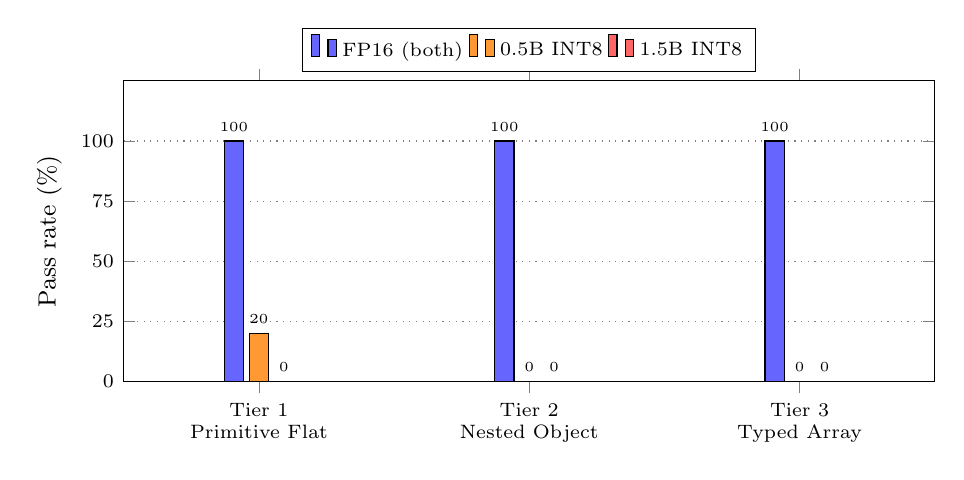
\begin{tikzpicture}
\begin{axis}[
  ybar,
  width=0.98\columnwidth, height=5.4cm,
  bar width=7pt,
  ylabel={Pass rate (\%)},
  ymin=0, ymax=125,
  ytick={0,25,50,75,100},
  symbolic x coords={t1,t2,t3},
  xtick=data,
  xticklabels={Tier 1\\Primitive Flat, Tier 2\\Nested Object, Tier 3\\Typed Array},
  x tick label style={align=center, font=\scriptsize},
  y tick label style={font=\scriptsize},
  ylabel style={font=\small},
  enlarge x limits=0.25,
  legend style={at={(0.5,1.03)}, anchor=south, legend columns=3, font=\scriptsize},
  nodes near coords,
  every node near coord/.append style={font=\tiny},
  ymajorgrids, grid style={dotted,gray}
]
\addplot[fill=blue!60]   coordinates {(t1,100) (t2,100) (t3,100)};
\addplot[fill=orange!80] coordinates {(t1,20) (t2,0) (t3,0)};
\addplot[fill=red!60]    coordinates {(t1,0) (t2,0) (t3,0)};
\legend{FP16 (both), 0.5B INT8, 1.5B INT8}
\end{axis}
\end{tikzpicture}
\caption{Structural pass rate by schema complexity tier. Only the 0.5B INT8 model passes any task, and only in Tier~1.}
\label{fig:tier_results}
\end{figure}

\section{Diagnostic Failure Taxonomy \& Qualitative Case Studies}

To make a diagnostic taxonomy of failure modes, we carefully categorized all 193 failure instances recorded on the INT8 evaluation logs. As shown in Table~\ref{tab:failure_taxonomy_distribution}, failures fall into three different categories.

\begin{table}[h]
\caption{Diagnostic Failure Taxonomy Breakdown ($N=193$ Total Failure Instances).}
\label{tab:failure_taxonomy_distribution}
\centering
\resizebox{\columnwidth}{!}{%
\begin{tabular}{lp{4.2cm}cc}
\toprule
\textbf{Failure Category} & \textbf{Primary Operational Manifestation} & \textbf{Count} & \textbf{Share (\%)} \\
\midrule
\errSyn & Unparseable JSON, conversational chatter, code fences, truncation & 131 & 67.9\% \\
\errField & Raw schema specification echoing, missing mandatory keys & 61 & 31.6\% \\
\errType & Valid JSON syntax with incorrect primitive value data types & 1 & 0.5\% \\
\midrule
\textbf{Total} & & \textbf{193} & \textbf{100.0\%} \\
\bottomrule
\end{tabular}}
\end{table}

% ---------- FIGURE 4: taxonomy ----------
\begin{figure}[!t]
\centering
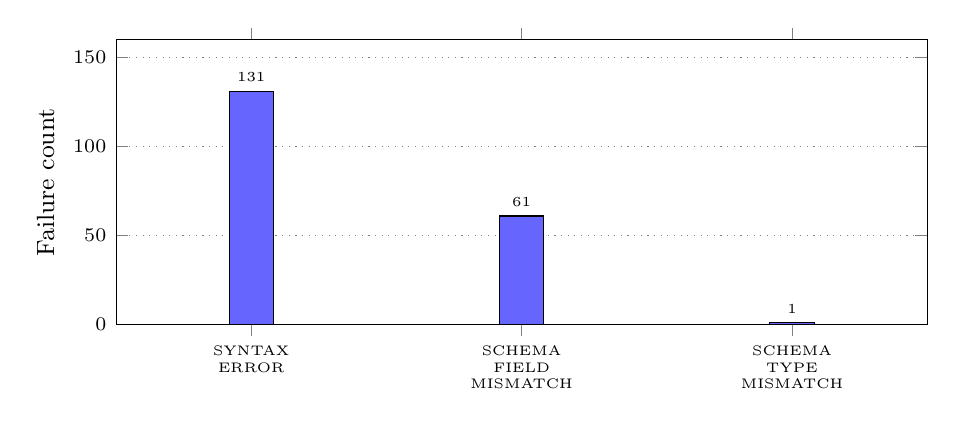
\begin{tikzpicture}
\begin{axis}[
  ybar,
  width=0.98\columnwidth, height=5.2cm,
  bar width=16pt,
  ylabel={Failure count},
  ymin=0, ymax=160,
  symbolic x coords={syn,fld,typ},
  xtick=data,
  xticklabels={SYNTAX\\ERROR, SCHEMA\\FIELD\\MISMATCH, SCHEMA\\TYPE\\MISMATCH},
  x tick label style={align=center, font=\tiny},
  y tick label style={font=\scriptsize},
  ylabel style={font=\small},
  enlarge x limits=0.25,
  nodes near coords={\pgfmathprintnumber{\pgfplotspointmeta}},
  every node near coord/.append style={font=\tiny},
  ymajorgrids, grid style={dotted,gray}
]
\addplot[fill=blue!60] coordinates {(syn,131) (fld,61) (typ,1)};
\end{axis}
\end{tikzpicture}
\caption{Distribution of the 193 INT8 failure instances by taxonomy category (67.9\%, 31.6\%, and 0.5\%).}
\label{fig:taxonomy}
\end{figure}

\subsection{Qualitative Analysis of Error Classes}

\subsubsection{\errSyn{} (67.9\% of Failures)}
The failure mode that dominated on both quantized models was the generation of unparseable strings ($67.9\%$). After doing qualitative checking, it is found that there are three primary manifestations:
\begin{enumerate}
    \item \textbf{Conversation preamble}: The model outputs conversation style text such as \emph{ "Here is the extracted JSON payload:" } before opening the JSON block.
    \item \textbf{Incorrectly closed code blocks}: Opening of a code block in markdown format (\verb|```json|) but the model stops generating and does not close the code block.
    \item \textbf{Conversation Trailing Disclaimers}: The model outputs valid JSON but then outputs bullet points/ disclaimers in conversation style.
\end{enumerate}

Second most common error type was schema mismatch (\subsubsection{\errField{} ($31.6\%$ of Failures)}). In particular, many ( $31.6\%$) quantised models failed to correctly populate values corresponding to the keys specified in the schema. Instead they simply repeated parts of the JSON schema itself, including ‘\textbf{’ keys, and ‘}’ values. We observed many repetitions of the keys ‘\texttt{"type": "object"}’, and ‘\texttt{"properties": \{...\}}’.

\subsubsection{\errType{} (0.5\% of Failures)}

Only very few type mismatch errors occurred ( 0.5\%). For those cases where a quantised model produced a syntactically correct JSON, the type of data stored within keys was consistent with the ground truth data in almost every case. This demonstrates that during quantisation, the structural syntactic routing (\emph{) is negatively impacted, but representation of concepts themselves (}) is not.

\section{Threats to Validity \& Protocol Scope}

Limitations and Scope of Findings:

\begin{enumerate}
    \item \textbf{Quantization Scheme Boundaries:} Our empirical results apply only to \textbf{PyTorch CPU per-tensor INT8 quantization} (\texttt{torch.ao.quantization.}\allowbreak\texttt{quantize\_dynamic}). They dont also do it for static post-training quantization that is guided by caliberation(e.g., GPTQ \cite{frantar2023gptq}, AWQ \cite{lin2024awq}), static block-wise quantization (GGUF k-quants), or quantization formats with outlier preservation (LLM.int8() \cite{dettmers2022llmint8}).
    \item \textbf{Decoding Paradigm Boundaries:} Experiments were only to \textbf{unconstrained autoregressive decoding}. Implementing schema-constrained decoding (e.g., Outlines \cite{willard2023outlines}) results in grammar token masking at inference time, guaranteeing 100\% syntactic compliance regardless of model precision.
    \item \textbf{Sample Size \& Model Generalizability:} While $N=100$ prompts provided statistical power ($p < 10^{-15}$) which is conclusive, future studies should evaluate additional model families (e.g., Llama-3, Mistral) and domain-specific schemas (e.g., medical records, financial compliance).
\end{enumerate}

\section{Prioritized Mitigation Strategies}

We rank three interventions by computational cost and structural information gain based on our empirical analysis:

\begin{enumerate}
    \item \textbf{Intervention 1: Schema-Constrained Decoding (Cost: Low | Gain: Immediate High):} make token masking by using context-free grammar state machines (e.g., Outlines \cite{willard2023outlines}) at the time of CPU inference. This completely removes \errSyn{} and \errField{} without need of weight retraining.
    \item \textbf{Intervention 2: Outlier-Aware Block-Wise Quantization (Cost: Medium | Gain: High):} Replace per-tensor CPU quantization with GGUF Q8\_0 or AWQ quantization featuring per-channel activation scaling, mitigating attention outlier clipping.
    \item \textbf{Intervention 3: Structure-Aware Quantization Calibration (Cost: High | Gain: High):} Use JSON extraction prompts in calibration datasets during post-training quantization so that sensitivity of attention weight over tokens is unmodified.
\end{enumerate}

\section{Conclusion}
In this paper, we introduced $D_{\text{formatting}}$ to measure how quantization causes structural formatting failures in small language models. Our tests on Qwen2.5-0.5B and Qwen2.5-1.5B show that dynamic INT8 CPU quantization leads to severe formatting drift ($-93.0\%$ to $-100.0\%$, $p < 10^{-15}$), which goes against the idea that extra parameter capacity protects the model. Looking closer at the errors, we found that unparseable syntax mistakes ($67.9\%$) and repeating the schema definition ($31.6\%$) make up most of the failures. Overall, unconstrained dynamic INT8 quantization does not work reliably for structured data extraction in live SLM microservices, meaning developers need to use grammar-constrained decoding or outlier-aware block-wise quantization instead.


\appendices

\section{Proof of Test Statistic Bound under Complete Collapse}
\begin{proof}
Consider the two-proportion pooled $Z$-statistic defined in Eq.~(\ref{eq:z_statistic_formula}):
\begin{equation}
    Z = \frac{P_2 - P_1}{\sqrt{\bar{p}(1 - \bar{p})\left(\frac{1}{N_1} + \frac{1}{N_2}\right)}}
\end{equation}
When $N_1 = N_2 = N$, $P_1 = 1.0$ (FP16 baseline pass rate), and $P_2 = 0.0$ (INT8 quantized pass rate), the pooled success proportion $\bar{p}$ evaluates to:
\begin{equation}
    \bar{p} = \frac{1.0 + 0.0}{2} = 0.5
\end{equation}
The denominator (Standard Error) evaluates to:
\begin{equation}
\begin{split}
    \text{SE} &= \sqrt{0.5 \times (1 - 0.5) \times \frac{2}{N}} = \sqrt{0.25 \times \frac{2}{N}} \\
              &= \sqrt{\frac{1}{2N}} = \frac{1}{\sqrt{2N}}
\end{split}
\end{equation}
Thus, the test statistic $Z$ is exact:
\begin{equation}
    Z = \frac{0.0 - 1.0}{1 / \sqrt{2N}} = -\sqrt{2N}
\end{equation}
For sample size $N=100$:
\begin{equation}
    Z = -\sqrt{200} \approx -14.1421356
\end{equation}
This establishes the exact mathematical lower bound for test statistic $Z$ under complete $100\%$ to $0\%$ structural pass collapse across equal sample sizes.
\end{proof}

\section{Exemplar Schema Complexity Tier Specifications}
Listing~\ref{lst:tier1_schema} demonstrates a representative Tier 1 Primitive Flat schema specification used in our benchmark dataset.

\begin{lstlisting}[language=json, float=tb, caption={Exemplar Tier 1 Primitive Flat Schema Specification.}, label={lst:tier1_schema}]
{
  "$schema": "http://json-schema.org/draft-07/schema#",
  "title": "UserScalarProfile",
  "type": "object",
  "properties": {
    "user_id": { "type": "integer" },
    "username": { "type": "string" },
    "is_active": { "type": "boolean" },
    "account_balance": { "type": "number" }
  },
  "required": ["user_id", "username", "is_active", "account_balance"],
  "additionalProperties": false
}
\end{lstlisting}

\nocite{shao2023omniquant}
\bibliographystyle{IEEEtran}
\bibliography{references}

\end{document}